\documentclass[paper=a4,fontsize=12pt]{scrartcl}
\usepackage{geometry}
\geometry{verbose, a4paper, tmargin=25mm, bmargin=25mm, lmargin=25mm, rmargin=25mm}

\usepackage[latin1]{inputenc}
\usepackage[ngerman]{babel}

\usepackage{fancyhdr} %Paket laden
\pagestyle{fancy} %eigener Seitenstil
\fancyhf{} %alle Kopf- und Fu�zeilenfelder bereinigen


\fancyhead[L]{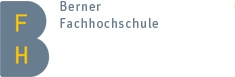
\includegraphics[width=1cm]{img/logo_bfh_de.jpg}} %Kopfzeile links
\fancyhead[C]{} %zentrierte Kopfzeile
\fancyhead[R]{Marco Berger, Andy Pollari} %Kopfzeile rechts
\renewcommand{\headrulewidth}{0.4pt} %obere Trennlinie
\fancyfoot[C]{\thepage} %Seitennummer
\renewcommand{\footrulewidth}{0.4pt} %untere Trennlinie
 
\begin{document}
\section*{Bildverschl�sselung mit Matlab}
\subsection*{Konzept}
In der heutigen Zeit werden kryptographische Verschl�sselungen in der Informatik immer wichtiger.
Dies kommt von dem immer gr�sseren Verlangen nach Privatsph�re und Datenschutz in der digitalen Welt.
In dieser Arbeit befassen wir uns mit der Anwendung verschiedener Verschl�sselungsalgorithmus
angewandt auf Bilder implementiert in Matlab. \\
Es ist zu erw�hnen, dass es grunds�tzlich zwei verschiedene Verschl�sselungsverfahren gibt:
\begin{itemize}
  \item Die synchrone Verschl�sselung
  \item Die asynchrone Verschl�sselung
\end{itemize}
Bei der synchronen Verschl�sselung wird mit einem Schl�ssel ver- wie auch entschl�sselt.
Bei der asynchronen hingegen gibt es zwei Schl�ssel: Einen �ffentlichen Schl�ssel zum verschl�sseln
und einen privaten Schl�ssel zum entschl�sseln. \\ \\
Es gibt verschiedene asymetrische Verschl�sselungsverfahren wie RSA, Merkle-Hellmann, RSA, \ldots \\
Auch bei den symetrischen Verschl�sselungsverfahren gibt es verschiedene wie DES, AES, One-Time-Pad, \ldots \\
Im Rahmen dieser Arbeit konzentrieren wir uns bei der synchronen Verschl�sselung auf das \textit{One-Time-Pad} 
und bei den asynchronen Verschl�sselungsverfahren auf RSA. \\ \\
In dieser Arbeit untersuchen wir einerseits die Performance verschiedener \\Verschl�sslungsalgorithmen
und ob man aus den verschl�sselten Bilddaten irgendwelche R�ckschl�sse ziehen kann.
Folgende Fragestellungen haben wir uns f�r diese Arbeit gestellt:
\begin{itemize}
  \item Wie unterschiedlich ist ein verschl�sseltes Bild mit dem Ausgangsbild?
  \item Kann man einen popul�res Bildformat wie JPEG oder PNG asynchron verschl�sseln, so dass
  das Bild immer noch korrekt interpretiert werden kann?
  \item Wie gut eignet sich Matlab f�r g�ngige Verschl�sselungsalgorithmen
\end{itemize}
Die Verschl�sselungen wenden wir auf JPEG Daten an.

 

\section*{Erwartete Resultate}
Uns ist bewusst, dass wir mit Matlab f�r eine Asynchrone Verschl�sselung keine
grossen Primzahlen nutzen k�nnen. Trotz relativ kleiner Primzahl, erwarten wir
bei der Asynchronen Verschl�sselung im Vergleich zu der synchronen Ver- und Entschl�sselung
grosse Performanceeinbussen. \\
Wir erwarten, dass wir bei einem Bildformat wie JPEG nur Darstellungsrelevanten
Daten ver- resp. entschl�sseln k�nnen.
Nach der Verschl�sselung kann das Bild auf keine Weise 
(ausser den nicht verschl�sselten Metadaten) mit dem Originalbild in Verbindung gebracht werden


\end{document}
